\chapter{\label{chap:anforderungen}Anforderungsdefinition}
Dieses Kapitel beschreibt die Anforderungen an eine Offline First Anwendung unter Berücksichtigung von Konfliktmanagement und Funktionalität. \todo{UI auch mit rein?}
Aus den oben genannten \hyperref[chap:szenarien]{Szenarien} werden im Folgenden die Anforderungen hergeleitet, die eine offlinefähige Anwendung erfüllen soll.
%
% Use Cases  \hyperref[sec:conflict]{oben}
%
\section{Anwendungsfälle}
Aus den in Kapitel \ref{chap:szenarien} erarbeiteten Szenarien ergeben sich die folgenden Use-Cases, die von einer offlinefähigen Anwendung erfüllt werden sollen. Die folgende Tabelle zeigt die Anwendungsfälle aus der Entwicklungsperspektive.
\begin{longtable}[c]{@{}
>{\columncolor[HTML]{CFFCC2}}l ll@{}}
\toprule
    \multicolumn{1}{p{0.1\textwidth}}{\cellcolor[HTML]{cffcc2}\textbf{ID}}
    & \multicolumn{1}{p{0.45\textwidth}}{\cellcolor[HTML]{cffcc2}\textbf{Anwendungsfall}}
    & \multicolumn{1}{p{0.45\textwidth}}{\cellcolor[HTML]{cffcc2}\textbf{Beschreibung}}\\ \hline
\endfirsthead
%
\endhead
%
  \multicolumn{1}{l}{\cellcolor[HTML]{cffcc2}\textbf{UC1}} &
  \multicolumn{1}{p{0.45\textwidth}}
  {Um die Anwendung auch ohne Internetzugang zu nutzen, sollen die Daten auch offline erreichbar sein.}
  & \multicolumn{1}{p{0.45\textwidth}}
  {Die Daten werden auf dem Server und lokal gespeichert. Lokal bedeutet in einer lokalen Datenbank oder im Browser (localStorage, IndexedDB usw.).}\\
  \midrule
  %
  \multicolumn{1}{l}{\cellcolor[HTML]{cffcc2}\textbf{UC2}} &
  \multicolumn{1}{p{0.45\textwidth}}
  {Die Anwendung soll die Kontaktliste schnell und effizient laden.}
  % {Um Datentraffic und Ladezeiten zu sparen / schnell und effizient möchte ich nur die Adressbucheinträge oder deren Aktualisierungen laden, die sich nicht schon auf dem Endgerät befinden.}
  & \multicolumn{1}{p{0.45\textwidth}}
  % {Es wird ermittelt welche Daten neu angelegt oder aktualisiert wurden. Dazu müssen sie sortierbar und versionierbar sein.}\\
  {Es werden nur Einträge oder deren Aktualisierungen geladen, die sich noch nicht auf dem Endgerät befinden.}\\
  \midrule
  %
  \multicolumn{1}{l}{\cellcolor[HTML]{cffcc2}\textbf{UC3}} &
  \multicolumn{1}{p{0.45\textwidth}}
  {Ich möchte Einträge immer und überall editieren können.}
  & \multicolumn{1}{p{0.45\textwidth}}
  {Jeder Eintrag muss identifizierbar und versionierbar sein.}\\
  \midrule
  %
  \multicolumn{1}{l}{\cellcolor[HTML]{cffcc2}\textbf{UC4}} &
  \multicolumn{1}{p{0.45\textwidth}}
  {Um jedem Adressbucheintrag Operationen zuzuweisen und einzelne Kontakte zu finden, möchte ich die Einträge identifizieren.}
  & \multicolumn{1}{p{0.45\textwidth}}
  {Jeder Eintrag bekommt zur eindeutigen Identifikation eine \gls{UUID} zugewiesen.}\\
  \midrule
  %
  \multicolumn{1}{l}{\cellcolor[HTML]{cffcc2}\textbf{UC5}} &
  \multicolumn{1}{p{0.45\textwidth}}
  {Um zu wissen ob, wie oft und wann ein Eintrag bearbeitet wurde, möchte ich die Einträge versionieren.}
  & \multicolumn{1}{p{0.45\textwidth}}
  {Jeder Eintrag bekommt ein Versionsattribut.}\\
  \midrule
  % UC6
  \multicolumn{1}{l}{\cellcolor[HTML]{cffcc2}\textbf{UC6}} &
  \multicolumn{1}{p{0.45\textwidth}}
  {Ich möchte dass alle Änderungen ankommen und keine Daten verloren gehen.}
  &
  \multicolumn{1}{p{0.45\textwidth}}
  {Wenn ein Konflikt auftritt, wird er effizient gespeichert (statt eine Version zu verwerfen).}\\
  \midrule
  % UC7
  \multicolumn{1}{l}{\cellcolor[HTML]{cffcc2}\textbf{UC7}} &
  \multicolumn{1}{p{0.45\textwidth}}
  {Ich weiß, Konflikte können immer auftreten, deswegen möchte ich mit ihnen umgehen können.}
  & \multicolumn{1}{p{0.45\textwidth}}
  {Konflikte werden effizient gespeichert, sodass sie nach und nach von NutzerInnen aufgelöst werden können.}\\
  % end
  \bottomrule \cellcolor[HTML]{FFFFFF}
  \vspace{0.1cm}\\
  \noalign{\hspace{0.0525\textwidth}\grayRule}
  \caption{Anwendungsfälle}
  \label{tab:uc}\\
\end{longtable}

Das in Abbildung \ref{fig:uc} gezeigte Use-Case-Diagramm veranschaulicht die in der obigen Tabelle \ref{tab:uc} aufgeführten Anwendungsfälle.
\begin{figure}[H]
    \centering
    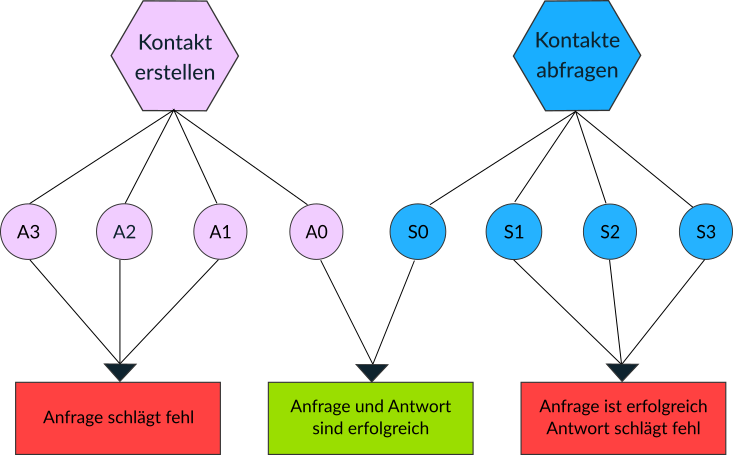
\includegraphics[width=\textwidth]{Szenarien}
    \grayRule
    \caption[Use-Case Diagramm]{Platzhalter für UC-Diagramm}
    \label{fig:uc}
\end{figure}
%
% Funktionalität
%
\section{Funktionalität}
Damit ein Datensatz, wie zum Beispiel ein Adressbucheintrag, offline erreichbar ist, sollte er wenigstens so lange auf dem Client gespeichert werden, bis er vollständig beim Server angekommen sind. Im aktuellen Anwendungsfall bedeutet das, es gibt zwei Kopien des Adressbucheintrags. Eine auf dem Anwendungsgerät, eine auf dem Server.\\
Jeder Fehlerfall muss kommuniziert werden. Wenn es konliktbehaftete Daten gibt muss dies mitgeteilt, und angeboten werden die Konflikte zu lösen (Welche Telefonnummer ist die richtige).\\
\begin{enumerate}
  \item Nur die Einträge laden die ich noch nicht hab
    \subitem kostet Bandbreite und Serverarbeitszeit
    \subitem doppelt (geladen)
    \subitem dauert länger (response)
  \item Einträge identifizieren
    \subitem Operationen müssen dem Objekt/Eintrag zugeordnet werden
  \item Einträge versionieren
  \item Delta berechnen
  \item lokal und auf dem Server gespeichert sein
  \item 2 Objekte mit derselben ID ? welches ist das aktuellste
  \item mehr als 2 Objekte mit derselben ID ? sortieren
  \item (Liste von inhaltsbasierten Versionen muss festgelegte Länge haben)
  \item Konflikte treten auf, deswegen müssen sie effizient gespeichert werden
  \item in Baumstruktur? So kann leicht zu einem konfliktfreiem Zustand (nur 1 Knoten) `navigiert` werden
  \item rekursiv lösen?
\end{enumerate}
\todo{Um Delta zu kalkulieren müssen Daten auf dem Client gespeichert werden (localStorage, lokale Datenbank oder Datei...) | Server muss die Daten sortieren können und in der Lage sein nur bestimmte Daten zu liefern.}
\todo{siehe Anforderungen \hyperref[sub:pwa]{PWA}?} Plus kein Datenverlust, und 'just work'\\
Daten sollen, sobald einmal geladen, auch offline verfügbar sein.
Daten sollen jederzeit (offline und online) lesbar und bearbeitbar (löschbar) sein.
\todo{Nochmal speziell auf Konfliktmanagement eingehen}
%
% UI
%
\section{User experience? Bedienoberfläche?}
\Gls{optimistic UI}\\
Einfache Liste mit Einträgen, editierbar, bei Konflikt: Dialog mit : welche Version möchtest du behalten?\\
\gls{UI} soll mich nicht mit Meldungen darüber nerven, dass ich offline bin\\
\gls{UI} soll sagen wenn es einen Konflikt gab / gibt und mich entscheiden lassen. Bzw ihn lösen lassen.
Auf keinen Fall selber lösen und mich nichts davon wissen lassen.\\
Im besten Fall soll die \gls{UI} mir sagen \b{warum} es zum Konflikt gekommen ist.
